\documentclass[11pt]{article}
\usepackage[review]{acl}
\usepackage{times}
\usepackage{latexsym}
\usepackage{amsmath}
\usepackage{amssymb}
\usepackage{graphicx}
\usepackage{booktabs}

\title{Death Avoidance Accounts for 90\% of the Routing Signal in LLM Agent Tool Use}

\author{Anonymous ACL submission}

\begin{document}
\maketitle
\begin{abstract}
Modular LLM agents that route between neural reasoning and deterministic computation promise improved reliability in rule-governed environments, yet understanding \emph{what} drives effective routing remains unclear. Per-step oracle labeling degenerates in sparse-reward settings---in ScienceWorld, 97.4\% of steps yield tied outcomes, rendering step-level analysis uninformative. We propose episode-level counterfactual analysis: running complete episodes under pure strategies and comparing final outcomes to derive per-episode routing labels. Across 245 episodes with a Qwen2.5-7B-Instruct backbone, death avoidance accounts for approximately 90\% of the routing signal (Death Avoidance Factor), with near-perfect cross-task correlation. These results indicate that deterministic computation's value is concentrated in catastrophic failure prevention rather than positive task guidance.
\end{abstract}

\section{Introduction}

When a Qwen2.5-7B-Instruct agent attempts to boil water in ScienceWorld \cite{scienceworld-2022}, it must track temperature thresholds, container states, and heat source interactions across dozens of steps. Internal LLM reasoning hallucinates these state transitions---predicting water has boiled when the stove was never activated---triggering agent death with a $-100$ penalty. Deterministic external computation (environment simulators, code interpreters) eliminates such hallucinations by executing exact state transitions. The natural question: when should an agent route computation externally versus reasoning internally?

Existing routing approaches \cite{toolformer-2024,art-2023,chameleon-2024} frame tool selection as a capability or efficiency decision---matching subtasks to tools that can solve them. This framing ignores a potentially dominant signal: routing to \emph{avoid catastrophic failure}. Understanding what routing actually learns requires counterfactual analysis, but the standard per-step oracle approach degenerates under sparse rewards. On ScienceWorld, where non-zero reward arrives only at episode termination, 97.4\% of steps produce tied intermediate scores under both strategies across 245 episodes---no step-level signal exists to train a router (\S\ref{sec:collection}).

We propose \emph{episode-level counterfactual analysis}: run complete episodes under pure-internal (ReAct~\cite{react-2023}) and pure-deterministic strategies, then compare episode outcomes to generate routing labels (\S\ref{sec:collection}). Across 11 ScienceWorld task types (245 episodes), the full deterministic advantage is $\Delta_{\text{full}} = +29.60$ points. Excluding death episodes, this gap collapses to $\Delta_{\text{nd}} = +2.84$---a Death Avoidance Factor (DAF; \S\ref{sec:daf}) of 90.41\%. The per-task correlation between death rate differential and performance gap is $r = 0.9698$ ($p = 8.12 \times 10^{-7}$), confirming death avoidance as the primary mechanism (\S\ref{sec:death-decomp}). Death rates differ sharply: 42.9\% for internal reasoning versus 16.3\% for deterministic computation. Of 245 episodes, 86 prefer deterministic, 9 prefer internal, and 150 show no preference---96.3\% of oracle decisions match always-deterministic (\S\ref{sec:baselines}).

Our contributions are twofold: (1)~an episode-level counterfactual methodology with death-aware labeling and the DAF metric, overcoming per-step oracle degeneracy (\S\ref{sec:collection}, \S\ref{sec:daf}); and (2)~the empirical finding that DAF = 90.41\% across 245 episodes, confirmed by router training as diagnostic probe (\S\ref{sec:router-diagnostic}).

\section{Method}

\subsection{Counterfactual Episode Collection}
\label{sec:collection}

For each task instance, we execute two complete episodes under identical initial conditions. The \emph{pure-internal} episode follows the ReAct paradigm \cite{react-2023}, where the LLM interleaves chain-of-thought reasoning with environment actions. The \emph{pure-deterministic} episode uses the environment simulator to compute exact state transitions. In both cases the LLM selects which action to take; deterministic computation replaces only the state-transition prediction---equivalent to giving the agent a perfect world model.

Each episode pair produces a tuple $(s^{\text{int}}, s^{\text{det}}, d^{\text{int}}, d^{\text{det}})$, where $s$ denotes the terminal score and $d \in \{0,1\}$ indicates agent death. Episodes are capped at 30 steps. The LLM backbone is Qwen2.5-7B-Instruct served via vLLM. ScienceWorld spans 30 task types with a $-100$ death penalty; after prescreening, we collect 245 episode pairs across 11 task types (20--40 per type).

\subsection{Death-Aware Labeling}
\label{sec:labeling}

Each counterfactual pair receives an episode-level routing label based on $(s^{\text{int}}, s^{\text{det}}, d^{\text{int}}, d^{\text{det}})$. Scores are integer-valued, so we use exact (in)equality. The label is assigned by four mutually exclusive cases:

\begin{enumerate}
    \item \textbf{Death asymmetry}: $d^{\text{int}} \neq d^{\text{det}}$ $\rightarrow$ surviving strategy preferred.
    \item \textbf{Both dead}: $d^{\text{int}} = d^{\text{det}} = 1$ $\rightarrow$ \texttt{no\_preference}.
    \item \textbf{Score gap}: both survive, $s^{\text{det}} \neq s^{\text{int}}$ $\rightarrow$ higher-scoring strategy preferred.
    \item \textbf{Tied alive}: both survive, $s^{\text{det}} = s^{\text{int}}$ $\rightarrow$ \texttt{no\_preference}.
\end{enumerate}

\subsection{Death Avoidance Factor}
\label{sec:daf}

To quantify the contribution of death avoidance to routing signal, we define the Death Avoidance Factor (DAF):
\begin{equation}
    \text{DAF} = 1 - \frac{\Delta_{\text{nd}}}{\Delta_{\text{full}}}
\end{equation}
where $\Delta_{\text{full}}$ is the mean score gap ($s^{\text{det}} - s^{\text{int}}$) across all episodes and $\Delta_{\text{nd}}$ excludes episodes where either strategy dies.

\section{Experiments}

\subsection{Death Avoidance Decomposition}
\label{sec:death-decomp}

\begin{figure}[t]
\centering
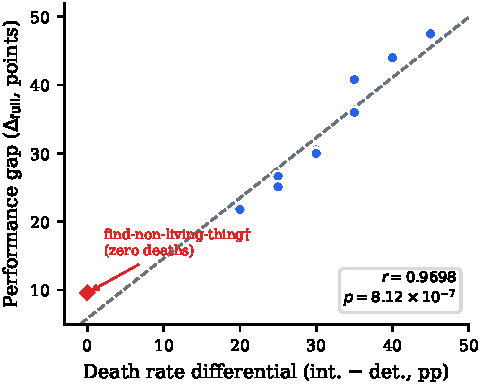
\includegraphics[width=\columnwidth]{fig1_daf_scatter.pdf}
\caption{Per-task death rate differential (internal minus deterministic) vs.\ $\Delta_{\text{full}}$. Each point represents one of 11 task types. Regression: $r = 0.9698$ ($p = 8.12 \times 10^{-7}$).}
\label{fig:decomposition}
\end{figure}

The full performance gap between deterministic and internal strategies across 245 episodes is $\Delta_{\text{full}} = +29.60$ points. Excluding all episodes where either strategy results in death, the gap collapses to $\Delta_{\text{nd}} = +2.84$. The resulting DAF (\S\ref{sec:daf}) is 90.41\%: approximately 90\% of the deterministic strategy's advantage is attributable to death avoidance.

This concentration is consistent across task types (Appendix~\ref{app:per-task}). The Pearson correlation between per-task death rate differential and $\Delta_{\text{full}}$ is $r = 0.9698$ ($p = 8.12 \times 10^{-7}$; Figure~\ref{fig:decomposition}). The internal strategy dies in 42.9\% of episodes versus 16.3\% for deterministic---a 2.6$\times$ ratio driving the bulk of the score difference.

The label distribution reflects this asymmetry: 86 \texttt{det\_preferred}, 9 \texttt{internal\_preferred}, 150 \texttt{no\_preference}. When internal reasoning does not cause death, it performs comparably to deterministic computation.

One task reveals residual non-death signal: \texttt{find-non-living-thing} ($n=40$) has zero deaths yet $\Delta_{\text{full}} = +9.58$, entirely from non-death differences. Among the 10 death-prone task types, however, death avoidance overwhelms non-death signal.

\subsection{Baselines}
\label{sec:baselines}

\begin{table}[t]
\centering
\small
\begin{tabular}{@{}lccc@{}}
\toprule
Strategy & Score & 95\% CI & Death \% \\
\midrule
Always-Internal & $-39.07$ & [$-46.40$, $-32.27$] & 42.9 \\
Always-Det. & $-9.47$ & [$-14.71$, $-4.29$] & 16.3 \\
Random & $-22.38$ & [$-28.67$, $-15.75$] & 27.8 \\
Oracle & $-6.58$ & [$-11.54$, $-1.70$] & 14.3 \\
\midrule
Trained Router & $-10.70$ & [$-16.33$, $-5.27$] & 17.6 \\
\bottomrule
\end{tabular}
\caption{Episode-weighted mean scores on ScienceWorld (11 task types, 245 episodes). 95\% Bootstrap CIs. The oracle selects the higher-scoring strategy per episode; 96.3\% of its decisions match always-deterministic.}
\label{tab:baselines}
\end{table}

Table~\ref{tab:baselines} reports episode-weighted mean scores and death rates. Always-deterministic ($-9.47$) outperforms always-internal ($-39.07$) by 29.60 points, consistent with $\Delta_{\text{full}}$. The oracle improves only modestly to $-6.58$, with 96.3\% of its decisions matching always-deterministic---\emph{oracle degeneracy} indicating the optimal routing policy closely resembles unconditional deterministic computation. Random routing ($-22.38$) falls between the two pure strategies.

Keyword-based routing fails: ScienceWorld's generic action verbs cause match rates to cluster at extremes (85.8\% or $<$5\%), degenerating to a pure strategy.

The trained router (\S\ref{sec:router-diagnostic}) scores $-10.70$, 1.23 points below always-deterministic, with comparable death rate (17.6\% vs.\ 16.3\%).

\subsection{Router Training as Diagnostic}
\label{sec:router-diagnostic}

We investigate whether episode-level counterfactual labels can train a step-level router, as a diagnostic probe rather than a routing system proposal.

\paragraph{Classification head.} A linear head appended to the LLM's hidden representations degenerates to always-deterministic (0\% internal recall) across all configurations (class weighting, focal loss, undersampling, temperature scaling).

\paragraph{Implicit router.} We fine-tune Qwen3-1.7B to internalize routing decisions. With GA=8 (effective batch 32), the model achieves 65.4\% generation accuracy and 51.5\% internal recall---the only non-degenerate configuration. GA=1 reaches 74.5\% logit accuracy but only 53.3\% generation accuracy (26.7\% internal recall)---a 21.2pp logit--generation gap indicating batch size governs transfer to generation.

Across four seeds (GA=8), balanced accuracy is $58.1 \pm 0.8\%$ (8 points above chance), with internal recall ranging 51.5--81.8\%. End-to-end, the router invokes the simulator 97.0\% of the time (Table~\ref{tab:baselines})---consistent with minimal routing structure beyond death avoidance.

\section{Related Work}

\paragraph{Tool-Use and Adaptive Computation.}
Toolformer \cite{toolformer-2024}, ART \cite{art-2023}, Chameleon \cite{chameleon-2024}, and ReTool \cite{retool-2026} learn \emph{which tool} to invoke but do not analyze what signal drives routing.
CogRouter \cite{cogrouter-2026} routes cognitive depth on ScienceWorld; ARES \cite{ares-2026} reduces token cost via per-step effort selection; Mixture-of-Recursions \cite{mixture-of-recursions-2025} applies adaptive depth via per-token recursive routing.
These route \emph{how much} to reason; we route \emph{which modality} and diagnose the signal composition---revealing ${\sim}90\%$ is death avoidance.

\paragraph{World Models and Agent Frameworks.}
ITP \cite{itp-2026} and Dyna-Think \cite{dynathink-2025} route to LLM-based world models inheriting hallucinations; our deterministic modality provides exact state transitions, with counterfactual analysis showing this exactness matters almost exclusively for death avoidance.
ReAct \cite{react-2023} serves as our internal-reasoning baseline; MTRouter \cite{mtrouter-2026} routes between LLMs for cost optimization.
Our work diagnoses \emph{what} a learned router captures---the answer is dominated by catastrophic-failure prevention.

\paragraph{Concurrent Work.}
Concurrent studies examine complementary aspects: cognitive illusions driving tool overuse \cite{tool-overuse-illusion-2026}, hidden-state encoding of tool-call decisions \cite{when2tool-2026}, a ``tool-use tax'' where tools are not always beneficial \cite{tool-use-tax-2026}, and necessity/utility/affordability evaluation \cite{to-call-or-not-2026}. Our death avoidance decomposition provides concrete quantification---${\sim}90\%$ of routing signal stems from catastrophic-failure prevention---grounding these frameworks in interactive-environment evidence.

\section{Conclusion}

We presented episode-level counterfactual analysis for diagnosing routing behavior in modular LLM agents. Applied to 245 episodes across 11 ScienceWorld task types, death avoidance accounts for 90.41\% of the routing signal ($\Delta_{\text{full}}$ = +29.60 vs.\ $\Delta_{\text{nd}}$ = +2.84), corroborated by near-perfect cross-task correlation ($r$ = 0.9698), oracle degeneracy (96.3\% agreement with always-deterministic), and near-random trained-router accuracy (58.1\%). A preliminary MATH pilot (50 problems) and an exploratory ALFWorld study (135 games) provide cross-environment evidence: MATH shows vanishing routing signal absent catastrophic failure, while ALFWorld exhibits the same deterministic-preferred asymmetry (25.9\% vs.\ 1.5\%)---consistent with death avoidance as the structural driver rather than a ScienceWorld artifact.


\section*{Limitations}

Our analysis uses a single benchmark (ScienceWorld) with a single LLM backbone (Qwen2.5-7B-Instruct), and generalization to other interactive environments and model scales remains to be established. The $-100$ death penalty may amplify DAF; environments with less catastrophic penalties could exhibit lower DAF, though the qualitative finding may still hold.

\paragraph{Cross-environment evidence.}
A preliminary 50-problem MATH Level~4--5 pilot, using code interpreter as the deterministic modality, provides initial evidence beyond ScienceWorld. Internal reasoning achieved 80\% accuracy versus 72\% for code interpreter, with 88\% of problems showing no modality preference (1 deterministic-preferred, 5 internal-preferred, 44 no-preference). In the absence of death risk, the routing signal vanishes or reverses---consistent with death avoidance as the primary driver. An exploratory ALFWorld study (135 games, 6 task types) shows a similar asymmetry: 25.9\% of episodes are deterministic-preferred versus 1.5\% internal-preferred, with deterministic success rate (27.4\%) far exceeding internal (3.0\%). While ALFWorld lacks ScienceWorld's explicit death penalty, task failure under internal reasoning is near-total, suggesting that catastrophic failure avoidance generalizes beyond environments with formal death mechanics.

\paragraph{Scope.}
Extending the counterfactual methodology to environments with graded failure costs, embodied agents, or multi-turn dialogue systems would clarify how broadly death avoidance accounts for apparent routing signal. Step-level labeling with denser rewards and the logit--generation gap in the implicit router are natural next steps. We audit labeling quality in Appendix~\ref{app:labeling}.

\section*{Ethics Statement}

This work uses ScienceWorld \cite{scienceworld-2022}, a publicly available text-based simulation environment, and does not involve human subjects or private data. All language models are accessed via standard APIs or publicly released weights. We report computational costs: approximately 40 GPU-hours on two RTX 5090 GPUs for data collection, router training, and evaluation.

\bibliography{references}

\appendix

\section{Labeling Quality Audit}
\label{app:labeling}

A potential concern is oracle circularity: whether episode-level labels reflect tie-breaking artifacts rather than genuine modality differences. We audit all 245 labels. Of the 150 \texttt{no\_preference} labels (61.2\%), 115 (46.9\%) are both-alive ties and 35 (14.3\%) are both-dead---all excluded from router training. The remaining 95 training labels are entirely genuine: 75 from death asymmetry (70 deterministic-preferred, 5 internal-preferred) and 20 from score comparison with both strategies surviving (16 deterministic-preferred, 4 internal-preferred). Zero labels depend on tie-breaking. Retraining the router using only death-asymmetry labels yields balanced accuracy of 57.3\%, within 1$\sigma$ of the full-label retrain (57.6 $\pm$ 0.5\%), confirming that score-comparison labels contribute negligible additional signal. The 97.4\% step-level tie rate (\S\ref{sec:collection}) further motivates episode-level over step-level labeling.

\section{Per-Task Decomposition}
\label{app:per-task}

\begin{table}[h]
\centering
\scriptsize
\setlength{\tabcolsep}{2.5pt}
\begin{tabular}{@{}lrrccc@{}}
\toprule
Task & $n$ & $\Delta_\text{full}$ & D\%\textsubscript{int} & D\%\textsubscript{det} & D / I / N \\
\midrule
id-life-stages-1       & 20  & $+47.50$ & 55   & 10   & 9 / 0 / 11  \\
lifespan-long          & 25  & $+44.00$ & 56   & 16   & 11 / 1 / 13 \\
lifespan-l-then-s      & 20  & $+40.80$ & 45   & 10   & 8 / 1 / 11  \\
inclined-plane         & 20  & $+36.00$ & 55   & 20   & 7 / 0 / 13  \\
freeze                 & 20  & $+30.50$ & 55   & 25   & 6 / 0 / 14  \\
meas-melt-point        & 20  & $+30.05$ & 55   & 25   & 6 / 0 / 14  \\
id-life-stages-2       & 20  & $+30.00$ & 50   & 20   & 6 / 0 / 14  \\
find-animal            & 20  & $+26.65$ & 50   & 25   & 5 / 0 / 15  \\
grow-fruit             & 20  & $+25.10$ & 45   & 20   & 6 / 1 / 13  \\
chem-mix               & 20  & $+21.80$ & 45   & 25   & 6 / 2 / 12  \\
\midrule
find-non-living$^\dagger$ & 40 & $+9.58$ & 0  & 0    & 16 / 4 / 20 \\
\midrule
\textbf{All (11 tasks)} & \textbf{245} & $\mathbf{+29.60}$ & \textbf{42.9} & \textbf{16.3} & \textbf{86 / 9 / 150} \\
\bottomrule
\end{tabular}
\caption{Per-task decomposition of the death avoidance effect. D\%: death rate for internal (int) and deterministic (det) strategies. D/I/N: episode labels (det-preferred / internal-preferred / no-preference). Sorted by $\Delta_{\text{full}}$ descending. $\dagger$\,Only task with zero deaths under both strategies.}
\label{tab:per-task}
\end{table}

\end{document}
